% Created by tikzDevice version 0.12.6 on 2025-02-04 13:53:36
% !TEX encoding = UTF-8 Unicode
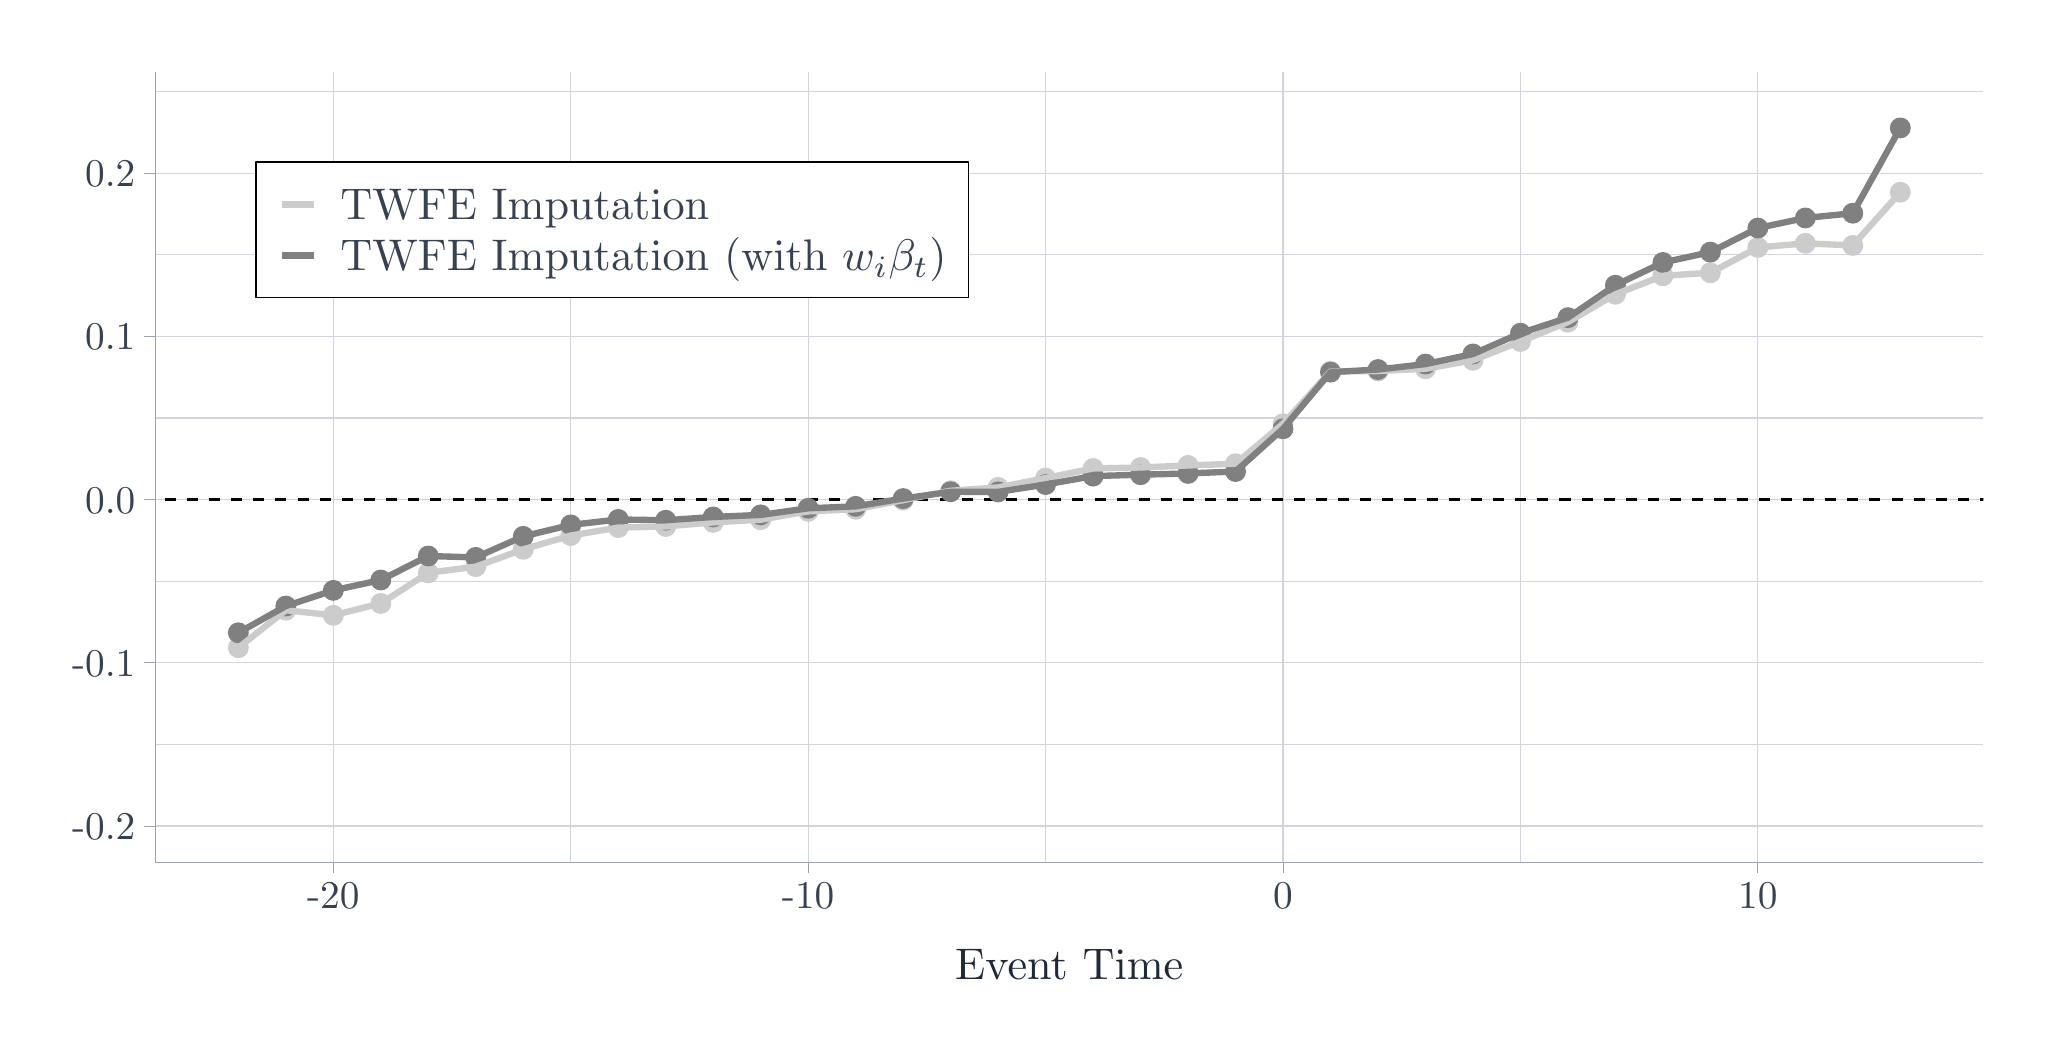
\begin{tikzpicture}[x=1pt,y=1pt]
\definecolor{fillColor}{RGB}{255,255,255}
\path[use as bounding box,fill=fillColor] (0,0) rectangle (722.70,361.35);
\begin{scope}
\path[clip] (  0.00,  0.00) rectangle (722.70,361.35);
\definecolor{drawColor}{RGB}{255,255,255}

\path[draw=drawColor,line width= 0.8pt,line join=round,line cap=round,fill=fillColor] (  0.00,  0.00) rectangle (722.70,361.35);
\end{scope}
\begin{scope}
\path[clip] ( 46.10, 59.89) rectangle (706.70,345.35);
\definecolor{drawColor}{RGB}{255,255,255}
\definecolor{fillColor}{RGB}{255,255,255}

\path[draw=drawColor,line width= 0.8pt,line join=round,line cap=round,fill=fillColor] ( 46.10, 59.89) rectangle (706.70,345.35);
\definecolor{drawColor}{RGB}{209,213,219}

\path[draw=drawColor,line width= 0.4pt,line join=round] ( 46.10,102.35) --
	(706.70,102.35);

\path[draw=drawColor,line width= 0.4pt,line join=round] ( 46.10,161.33) --
	(706.70,161.33);

\path[draw=drawColor,line width= 0.4pt,line join=round] ( 46.10,220.31) --
	(706.70,220.31);

\path[draw=drawColor,line width= 0.4pt,line join=round] ( 46.10,279.29) --
	(706.70,279.29);

\path[draw=drawColor,line width= 0.4pt,line join=round] ( 46.10,338.27) --
	(706.70,338.27);

\path[draw=drawColor,line width= 0.4pt,line join=round] (196.24, 59.89) --
	(196.24,345.35);

\path[draw=drawColor,line width= 0.4pt,line join=round] (367.82, 59.89) --
	(367.82,345.35);

\path[draw=drawColor,line width= 0.4pt,line join=round] (539.41, 59.89) --
	(539.41,345.35);

\path[draw=drawColor,line width= 0.4pt,line join=round] ( 46.10, 72.86) --
	(706.70, 72.86);

\path[draw=drawColor,line width= 0.4pt,line join=round] ( 46.10,131.84) --
	(706.70,131.84);

\path[draw=drawColor,line width= 0.4pt,line join=round] ( 46.10,190.82) --
	(706.70,190.82);

\path[draw=drawColor,line width= 0.4pt,line join=round] ( 46.10,249.80) --
	(706.70,249.80);

\path[draw=drawColor,line width= 0.4pt,line join=round] ( 46.10,308.78) --
	(706.70,308.78);

\path[draw=drawColor,line width= 0.4pt,line join=round] (110.45, 59.89) --
	(110.45,345.35);

\path[draw=drawColor,line width= 0.4pt,line join=round] (282.03, 59.89) --
	(282.03,345.35);

\path[draw=drawColor,line width= 0.4pt,line join=round] (453.61, 59.89) --
	(453.61,345.35);

\path[draw=drawColor,line width= 0.4pt,line join=round] (625.20, 59.89) --
	(625.20,345.35);
\definecolor{drawColor}{RGB}{0,0,0}

\path[draw=drawColor,line width= 0.9pt,dash pattern=on 4pt off 4pt ,line join=round] (-614.49,190.82) -- (1367.30,190.82);
\definecolor{drawColor}{gray}{0.80}
\definecolor{fillColor}{gray}{0.80}

\path[draw=drawColor,line width= 0.4pt,line join=round,line cap=round,fill=fillColor] ( 76.13,137.29) circle (  3.57);

\path[draw=drawColor,line width= 0.4pt,line join=round,line cap=round,fill=fillColor] ( 93.29,150.85) circle (  3.57);

\path[draw=drawColor,line width= 0.4pt,line join=round,line cap=round,fill=fillColor] (110.45,149.00) circle (  3.57);

\path[draw=drawColor,line width= 0.4pt,line join=round,line cap=round,fill=fillColor] (127.61,153.30) circle (  3.57);

\path[draw=drawColor,line width= 0.4pt,line join=round,line cap=round,fill=fillColor] (144.76,164.35) circle (  3.57);

\path[draw=drawColor,line width= 0.4pt,line join=round,line cap=round,fill=fillColor] (161.92,166.60) circle (  3.57);

\path[draw=drawColor,line width= 0.4pt,line join=round,line cap=round,fill=fillColor] (179.08,172.86) circle (  3.57);

\path[draw=drawColor,line width= 0.4pt,line join=round,line cap=round,fill=fillColor] (196.24,177.83) circle (  3.57);

\path[draw=drawColor,line width= 0.4pt,line join=round,line cap=round,fill=fillColor] (213.40,180.71) circle (  3.57);

\path[draw=drawColor,line width= 0.4pt,line join=round,line cap=round,fill=fillColor] (230.56,181.10) circle (  3.57);

\path[draw=drawColor,line width= 0.4pt,line join=round,line cap=round,fill=fillColor] (247.71,182.58) circle (  3.57);

\path[draw=drawColor,line width= 0.4pt,line join=round,line cap=round,fill=fillColor] (264.87,183.55) circle (  3.57);

\path[draw=drawColor,line width= 0.4pt,line join=round,line cap=round,fill=fillColor] (282.03,186.57) circle (  3.57);

\path[draw=drawColor,line width= 0.4pt,line join=round,line cap=round,fill=fillColor] (299.19,187.33) circle (  3.57);

\path[draw=drawColor,line width= 0.4pt,line join=round,line cap=round,fill=fillColor] (316.35,190.62) circle (  3.57);

\path[draw=drawColor,line width= 0.4pt,line join=round,line cap=round,fill=fillColor] (333.51,194.01) circle (  3.57);

\path[draw=drawColor,line width= 0.4pt,line join=round,line cap=round,fill=fillColor] (350.66,195.22) circle (  3.57);

\path[draw=drawColor,line width= 0.4pt,line join=round,line cap=round,fill=fillColor] (367.82,198.60) circle (  3.57);

\path[draw=drawColor,line width= 0.4pt,line join=round,line cap=round,fill=fillColor] (384.98,202.06) circle (  3.57);

\path[draw=drawColor,line width= 0.4pt,line join=round,line cap=round,fill=fillColor] (402.14,202.42) circle (  3.57);

\path[draw=drawColor,line width= 0.4pt,line join=round,line cap=round,fill=fillColor] (419.30,203.15) circle (  3.57);

\path[draw=drawColor,line width= 0.4pt,line join=round,line cap=round,fill=fillColor] (436.46,203.77) circle (  3.57);

\path[draw=drawColor,line width= 0.4pt,line join=round,line cap=round,fill=fillColor] (453.61,218.23) circle (  3.57);

\path[draw=drawColor,line width= 0.4pt,line join=round,line cap=round,fill=fillColor] (470.77,237.11) circle (  3.57);

\path[draw=drawColor,line width= 0.4pt,line join=round,line cap=round,fill=fillColor] (487.93,237.26) circle (  3.57);

\path[draw=drawColor,line width= 0.4pt,line join=round,line cap=round,fill=fillColor] (505.09,238.10) circle (  3.57);

\path[draw=drawColor,line width= 0.4pt,line join=round,line cap=round,fill=fillColor] (522.25,241.15) circle (  3.57);

\path[draw=drawColor,line width= 0.4pt,line join=round,line cap=round,fill=fillColor] (539.41,247.95) circle (  3.57);

\path[draw=drawColor,line width= 0.4pt,line join=round,line cap=round,fill=fillColor] (556.56,254.94) circle (  3.57);

\path[draw=drawColor,line width= 0.4pt,line join=round,line cap=round,fill=fillColor] (573.72,265.02) circle (  3.57);

\path[draw=drawColor,line width= 0.4pt,line join=round,line cap=round,fill=fillColor] (590.88,271.69) circle (  3.57);

\path[draw=drawColor,line width= 0.4pt,line join=round,line cap=round,fill=fillColor] (608.04,272.77) circle (  3.57);

\path[draw=drawColor,line width= 0.4pt,line join=round,line cap=round,fill=fillColor] (625.20,281.92) circle (  3.57);

\path[draw=drawColor,line width= 0.4pt,line join=round,line cap=round,fill=fillColor] (642.36,283.42) circle (  3.57);

\path[draw=drawColor,line width= 0.4pt,line join=round,line cap=round,fill=fillColor] (659.51,282.66) circle (  3.57);

\path[draw=drawColor,line width= 0.4pt,line join=round,line cap=round,fill=fillColor] (676.67,301.88) circle (  3.57);
\definecolor{drawColor}{gray}{0.50}
\definecolor{fillColor}{gray}{0.50}

\path[draw=drawColor,line width= 0.4pt,line join=round,line cap=round,fill=fillColor] ( 76.13,142.68) circle (  3.57);

\path[draw=drawColor,line width= 0.4pt,line join=round,line cap=round,fill=fillColor] ( 93.29,152.35) circle (  3.57);

\path[draw=drawColor,line width= 0.4pt,line join=round,line cap=round,fill=fillColor] (110.45,158.02) circle (  3.57);

\path[draw=drawColor,line width= 0.4pt,line join=round,line cap=round,fill=fillColor] (127.61,161.76) circle (  3.57);

\path[draw=drawColor,line width= 0.4pt,line join=round,line cap=round,fill=fillColor] (144.76,170.43) circle (  3.57);

\path[draw=drawColor,line width= 0.4pt,line join=round,line cap=round,fill=fillColor] (161.92,169.93) circle (  3.57);

\path[draw=drawColor,line width= 0.4pt,line join=round,line cap=round,fill=fillColor] (179.08,177.53) circle (  3.57);

\path[draw=drawColor,line width= 0.4pt,line join=round,line cap=round,fill=fillColor] (196.24,181.67) circle (  3.57);

\path[draw=drawColor,line width= 0.4pt,line join=round,line cap=round,fill=fillColor] (213.40,183.64) circle (  3.57);

\path[draw=drawColor,line width= 0.4pt,line join=round,line cap=round,fill=fillColor] (230.56,183.36) circle (  3.57);

\path[draw=drawColor,line width= 0.4pt,line join=round,line cap=round,fill=fillColor] (247.71,184.54) circle (  3.57);

\path[draw=drawColor,line width= 0.4pt,line join=round,line cap=round,fill=fillColor] (264.87,185.29) circle (  3.57);

\path[draw=drawColor,line width= 0.4pt,line join=round,line cap=round,fill=fillColor] (282.03,187.67) circle (  3.57);

\path[draw=drawColor,line width= 0.4pt,line join=round,line cap=round,fill=fillColor] (299.19,188.38) circle (  3.57);

\path[draw=drawColor,line width= 0.4pt,line join=round,line cap=round,fill=fillColor] (316.35,191.19) circle (  3.57);

\path[draw=drawColor,line width= 0.4pt,line join=round,line cap=round,fill=fillColor] (333.51,193.64) circle (  3.57);

\path[draw=drawColor,line width= 0.4pt,line join=round,line cap=round,fill=fillColor] (350.66,193.60) circle (  3.57);

\path[draw=drawColor,line width= 0.4pt,line join=round,line cap=round,fill=fillColor] (367.82,196.27) circle (  3.57);

\path[draw=drawColor,line width= 0.4pt,line join=round,line cap=round,fill=fillColor] (384.98,199.31) circle (  3.57);

\path[draw=drawColor,line width= 0.4pt,line join=round,line cap=round,fill=fillColor] (402.14,199.81) circle (  3.57);

\path[draw=drawColor,line width= 0.4pt,line join=round,line cap=round,fill=fillColor] (419.30,200.27) circle (  3.57);

\path[draw=drawColor,line width= 0.4pt,line join=round,line cap=round,fill=fillColor] (436.46,200.96) circle (  3.57);

\path[draw=drawColor,line width= 0.4pt,line join=round,line cap=round,fill=fillColor] (453.61,216.40) circle (  3.57);

\path[draw=drawColor,line width= 0.4pt,line join=round,line cap=round,fill=fillColor] (470.77,236.87) circle (  3.57);

\path[draw=drawColor,line width= 0.4pt,line join=round,line cap=round,fill=fillColor] (487.93,237.82) circle (  3.57);

\path[draw=drawColor,line width= 0.4pt,line join=round,line cap=round,fill=fillColor] (505.09,239.79) circle (  3.57);

\path[draw=drawColor,line width= 0.4pt,line join=round,line cap=round,fill=fillColor] (522.25,243.43) circle (  3.57);

\path[draw=drawColor,line width= 0.4pt,line join=round,line cap=round,fill=fillColor] (539.41,250.94) circle (  3.57);

\path[draw=drawColor,line width= 0.4pt,line join=round,line cap=round,fill=fillColor] (556.56,256.56) circle (  3.57);

\path[draw=drawColor,line width= 0.4pt,line join=round,line cap=round,fill=fillColor] (573.72,268.28) circle (  3.57);

\path[draw=drawColor,line width= 0.4pt,line join=round,line cap=round,fill=fillColor] (590.88,276.49) circle (  3.57);

\path[draw=drawColor,line width= 0.4pt,line join=round,line cap=round,fill=fillColor] (608.04,280.24) circle (  3.57);

\path[draw=drawColor,line width= 0.4pt,line join=round,line cap=round,fill=fillColor] (625.20,288.94) circle (  3.57);

\path[draw=drawColor,line width= 0.4pt,line join=round,line cap=round,fill=fillColor] (642.36,292.58) circle (  3.57);

\path[draw=drawColor,line width= 0.4pt,line join=round,line cap=round,fill=fillColor] (659.51,294.30) circle (  3.57);

\path[draw=drawColor,line width= 0.4pt,line join=round,line cap=round,fill=fillColor] (676.67,325.12) circle (  3.57);
\definecolor{drawColor}{gray}{0.80}

\path[draw=drawColor,line width= 2.3pt,line join=round] ( 76.13,137.29) --
	( 93.29,150.85) --
	(110.45,149.00) --
	(127.61,153.30) --
	(144.76,164.35) --
	(161.92,166.60) --
	(179.08,172.86) --
	(196.24,177.83) --
	(213.40,180.71) --
	(230.56,181.10) --
	(247.71,182.58) --
	(264.87,183.55) --
	(282.03,186.57) --
	(299.19,187.33) --
	(316.35,190.62) --
	(333.51,194.01) --
	(350.66,195.22) --
	(367.82,198.60) --
	(384.98,202.06) --
	(402.14,202.42) --
	(419.30,203.15) --
	(436.46,203.77) --
	(453.61,218.23) --
	(470.77,237.11) --
	(487.93,237.26) --
	(505.09,238.10) --
	(522.25,241.15) --
	(539.41,247.95) --
	(556.56,254.94) --
	(573.72,265.02) --
	(590.88,271.69) --
	(608.04,272.77) --
	(625.20,281.92) --
	(642.36,283.42) --
	(659.51,282.66) --
	(676.67,301.88);
\definecolor{drawColor}{gray}{0.50}

\path[draw=drawColor,line width= 2.3pt,line join=round] ( 76.13,142.68) --
	( 93.29,152.35) --
	(110.45,158.02) --
	(127.61,161.76) --
	(144.76,170.43) --
	(161.92,169.93) --
	(179.08,177.53) --
	(196.24,181.67) --
	(213.40,183.64) --
	(230.56,183.36) --
	(247.71,184.54) --
	(264.87,185.29) --
	(282.03,187.67) --
	(299.19,188.38) --
	(316.35,191.19) --
	(333.51,193.64) --
	(350.66,193.60) --
	(367.82,196.27) --
	(384.98,199.31) --
	(402.14,199.81) --
	(419.30,200.27) --
	(436.46,200.96) --
	(453.61,216.40) --
	(470.77,236.87) --
	(487.93,237.82) --
	(505.09,239.79) --
	(522.25,243.43) --
	(539.41,250.94) --
	(556.56,256.56) --
	(573.72,268.28) --
	(590.88,276.49) --
	(608.04,280.24) --
	(625.20,288.94) --
	(642.36,292.58) --
	(659.51,294.30) --
	(676.67,325.12);
\end{scope}
\begin{scope}
\path[clip] (  0.00,  0.00) rectangle (722.70,361.35);
\definecolor{drawColor}{RGB}{156,163,175}

\path[draw=drawColor,line width= 0.3pt,line join=round] ( 46.10, 59.89) --
	( 46.10,345.35);
\end{scope}
\begin{scope}
\path[clip] (  0.00,  0.00) rectangle (722.70,361.35);
\definecolor{drawColor}{RGB}{55,65,81}

\node[text=drawColor,anchor=base east,inner sep=0pt, outer sep=0pt, scale=  1.42] at ( 38.90, 67.97) {-0.2};

\node[text=drawColor,anchor=base east,inner sep=0pt, outer sep=0pt, scale=  1.42] at ( 38.90,126.95) {-0.1};

\node[text=drawColor,anchor=base east,inner sep=0pt, outer sep=0pt, scale=  1.42] at ( 38.90,185.93) {0.0};

\node[text=drawColor,anchor=base east,inner sep=0pt, outer sep=0pt, scale=  1.42] at ( 38.90,244.91) {0.1};

\node[text=drawColor,anchor=base east,inner sep=0pt, outer sep=0pt, scale=  1.42] at ( 38.90,303.89) {0.2};
\end{scope}
\begin{scope}
\path[clip] (  0.00,  0.00) rectangle (722.70,361.35);
\definecolor{drawColor}{RGB}{156,163,175}

\path[draw=drawColor,line width= 0.3pt,line join=round] ( 42.10, 72.86) --
	( 46.10, 72.86);

\path[draw=drawColor,line width= 0.3pt,line join=round] ( 42.10,131.84) --
	( 46.10,131.84);

\path[draw=drawColor,line width= 0.3pt,line join=round] ( 42.10,190.82) --
	( 46.10,190.82);

\path[draw=drawColor,line width= 0.3pt,line join=round] ( 42.10,249.80) --
	( 46.10,249.80);

\path[draw=drawColor,line width= 0.3pt,line join=round] ( 42.10,308.78) --
	( 46.10,308.78);
\end{scope}
\begin{scope}
\path[clip] (  0.00,  0.00) rectangle (722.70,361.35);
\definecolor{drawColor}{RGB}{156,163,175}

\path[draw=drawColor,line width= 0.3pt,line join=round] ( 46.10, 59.89) --
	(706.70, 59.89);
\end{scope}
\begin{scope}
\path[clip] (  0.00,  0.00) rectangle (722.70,361.35);
\definecolor{drawColor}{RGB}{156,163,175}

\path[draw=drawColor,line width= 0.3pt,line join=round] (110.45, 55.89) --
	(110.45, 59.89);

\path[draw=drawColor,line width= 0.3pt,line join=round] (282.03, 55.89) --
	(282.03, 59.89);

\path[draw=drawColor,line width= 0.3pt,line join=round] (453.61, 55.89) --
	(453.61, 59.89);

\path[draw=drawColor,line width= 0.3pt,line join=round] (625.20, 55.89) --
	(625.20, 59.89);
\end{scope}
\begin{scope}
\path[clip] (  0.00,  0.00) rectangle (722.70,361.35);
\definecolor{drawColor}{RGB}{55,65,81}

\node[text=drawColor,anchor=base,inner sep=0pt, outer sep=0pt, scale=  1.42] at (110.45, 42.89) {-20};

\node[text=drawColor,anchor=base,inner sep=0pt, outer sep=0pt, scale=  1.42] at (282.03, 42.89) {-10};

\node[text=drawColor,anchor=base,inner sep=0pt, outer sep=0pt, scale=  1.42] at (453.61, 42.89) {0};

\node[text=drawColor,anchor=base,inner sep=0pt, outer sep=0pt, scale=  1.42] at (625.20, 42.89) {10};
\end{scope}
\begin{scope}
\path[clip] (  0.00,  0.00) rectangle (722.70,361.35);
\definecolor{drawColor}{RGB}{31,41,55}

\node[text=drawColor,anchor=base,inner sep=0pt, outer sep=0pt, scale=  1.60] at (376.40, 17.56) {Event Time};
\end{scope}
\begin{scope}
\path[clip] (  0.00,  0.00) rectangle (722.70,361.35);
\definecolor{drawColor}{RGB}{0,0,0}
\definecolor{fillColor}{RGB}{255,255,255}

\path[draw=drawColor,line width= 0.6pt,line join=round,line cap=round,fill=fillColor] ( 82.54,263.80) rectangle (339.97,312.71);
\end{scope}
\begin{scope}
\path[clip] (  0.00,  0.00) rectangle (722.70,361.35);
\definecolor{drawColor}{RGB}{255,255,255}
\definecolor{fillColor}{RGB}{255,255,255}

\path[draw=drawColor,line width= 0.8pt,line join=round,line cap=round,fill=fillColor] ( 90.54,290.26) rectangle (104.99,304.71);
\end{scope}
\begin{scope}
\path[clip] (  0.00,  0.00) rectangle (722.70,361.35);
\definecolor{drawColor}{gray}{0.80}
\definecolor{fillColor}{gray}{0.80}

\path[draw=drawColor,line width= 0.4pt,line join=round,line cap=round,fill=fillColor] ( 97.77,297.48) circle (  0.36);
\end{scope}
\begin{scope}
\path[clip] (  0.00,  0.00) rectangle (722.70,361.35);
\definecolor{drawColor}{gray}{0.80}

\path[draw=drawColor,line width= 2.5pt,line join=round] ( 91.98,297.48) -- (103.55,297.48);
\end{scope}
\begin{scope}
\path[clip] (  0.00,  0.00) rectangle (722.70,361.35);
\definecolor{drawColor}{RGB}{255,255,255}
\definecolor{fillColor}{RGB}{255,255,255}

\path[draw=drawColor,line width= 0.8pt,line join=round,line cap=round,fill=fillColor] ( 90.54,271.80) rectangle (104.99,286.26);
\end{scope}
\begin{scope}
\path[clip] (  0.00,  0.00) rectangle (722.70,361.35);
\definecolor{drawColor}{gray}{0.50}
\definecolor{fillColor}{gray}{0.50}

\path[draw=drawColor,line width= 0.4pt,line join=round,line cap=round,fill=fillColor] ( 97.77,279.03) circle (  0.36);
\end{scope}
\begin{scope}
\path[clip] (  0.00,  0.00) rectangle (722.70,361.35);
\definecolor{drawColor}{gray}{0.50}

\path[draw=drawColor,line width= 2.5pt,line join=round] ( 91.98,279.03) -- (103.55,279.03);
\end{scope}
\begin{scope}
\path[clip] (  0.00,  0.00) rectangle (722.70,361.35);
\definecolor{drawColor}{RGB}{55,65,81}

\node[text=drawColor,anchor=base west,inner sep=0pt, outer sep=0pt, scale=  1.60] at (112.99,291.97) {TWFE Imputation};
\end{scope}
\begin{scope}
\path[clip] (  0.00,  0.00) rectangle (722.70,361.35);
\definecolor{drawColor}{RGB}{55,65,81}

\node[text=drawColor,anchor=base west,inner sep=0pt, outer sep=0pt, scale=  1.60] at (112.99,273.52) {TWFE Imputation (with $w_i \beta_t$)};
\end{scope}
\end{tikzpicture}
